\section{Summary}


Monitoring fish stocks is a critical component of sustainable fisheries management in the Southern Gulf of St. Lawrence.
One key aspect of this work is understanding the population dynamics of various fish stocks, which involves accurate age determination.
Age data are essential for modeling growth patterns, understanding reproduction, and assessing the health and sustainability of fish populations.
The primary objective of this project is to develop and implement a machine learning-based predictive model capable of estimating the age of fish from otolith images.
This model will automate the process of age determination, reduce the potential for human error, and provide quicker assessments for large datasets.

Fish age is commonly determined by examining biological materials such as otoliths (inner ear bones) and scales.
These materials exhibit growth rings, or \enquote{annuli} (Figure~\ref{fig:plaice_oto_example} and Figure~\ref{fig:herring_oto_example}), which can be counted similarly to tree rings.
Each ring represents a period of growth, typically corresponding to one year in the life of the fish.
However, manually counting these rings can be time-consuming, subjective, and prone to human error.

The development of an automated system for predicting fish age based on otolith images would significantly improve the accuracy and speed of age estimation.

\subsection{Data source}

The data used for this analysis originate from archives of images taken of otoliths from two Atlantic Canadian species of fish: Atlantic Herring and American Plaice.
While these archives are unpublished, some of the details about how the otoliths were collected, preserved and imaged are available on the Government of Canada's Open Data Portal ~\cite{ogp_plaice}.
The dataset contained ages that were evaluated by human experts and which are actively used in annual population models for the two species in question.

\subsection{Analysis}

First, we aimed to build a simple predictive model that integrates the image data with the metadata measurements, with the goal of outperforming the metadata alone.
Comparison of SVM regressor (SVR), Elastic Net, Decision Tree, Random Forest, XGBoost, Voting, and Stacking (combining SVR, ElasticNet, Decision Tree, Random Forest, and XGBoost with the secondary model as indicated in the tables below) models were performed on the datasets.
A randomized grid search was performed separately for each model to determine the optimal hyperparameters before comparing the models.
Metrics such as Mean Squared Error (MSE), Root Mean Squared Error (RMSE), R-squared (R\textsuperscript{2}) were used as key evaluators.

Next, we built models on the integrated metadata and image data aiming for better performance but applying a PCA transformation on the image data, preserving 95\% of the variance.
As a result, the dimensionality of the image data was reduced from 4,096 pixels to 340 dimensions

Finally, we explored a Convolutional Neural Network (CNN) model to further enhance our predictive performance.
The CNN model is designed to automatically learn relevant features from the otolith images, which is particularly useful in identifying the age-related annuli in the images.
The CNN architecture used in this analysis consists of several convolutional and pooling layers, followed by fully connected layers that allow for regression of the fish age.

\subsection{Conclusions}

While we took steps in the right direction with our project, we did not produce a model that would have any value in a production context.
Our analysis highlights the potential for convolutional neutral networks (CNNs) to perform well in situations where the data is very large and complex.
More work is needed for determining how CNN models can be fine-tuned to determine age from otolith images.

For future analyses, we plan to explore tools designed for efficiently handling large datasets through distributed computing.
Instead of relying on a local setup like Jupyter Notebooks, we could leverage platforms that support scalable computation across multiple servers.
This would enable parallel processing, significantly improving the speed of data analysis and model training.
As a result, we could minimize the need to downsize images, preserving model accuracy without excessive computational time.


\begin{figure}
    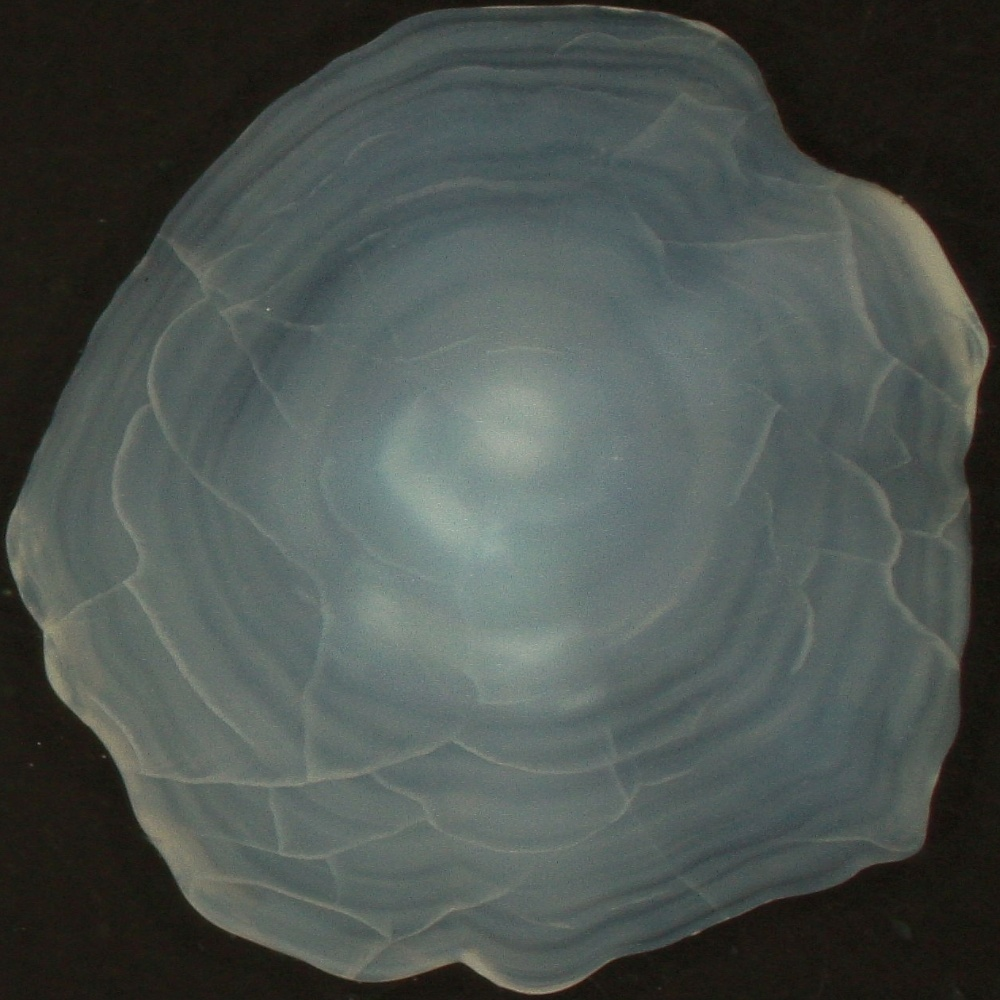
\includegraphics[width=\linewidth]{plaice_otolith_example}
    \caption{An example of an otolith image taken from an American Plaice.}
    \label{fig:plaice_oto_example}
\end{figure}

\begin{figure}
    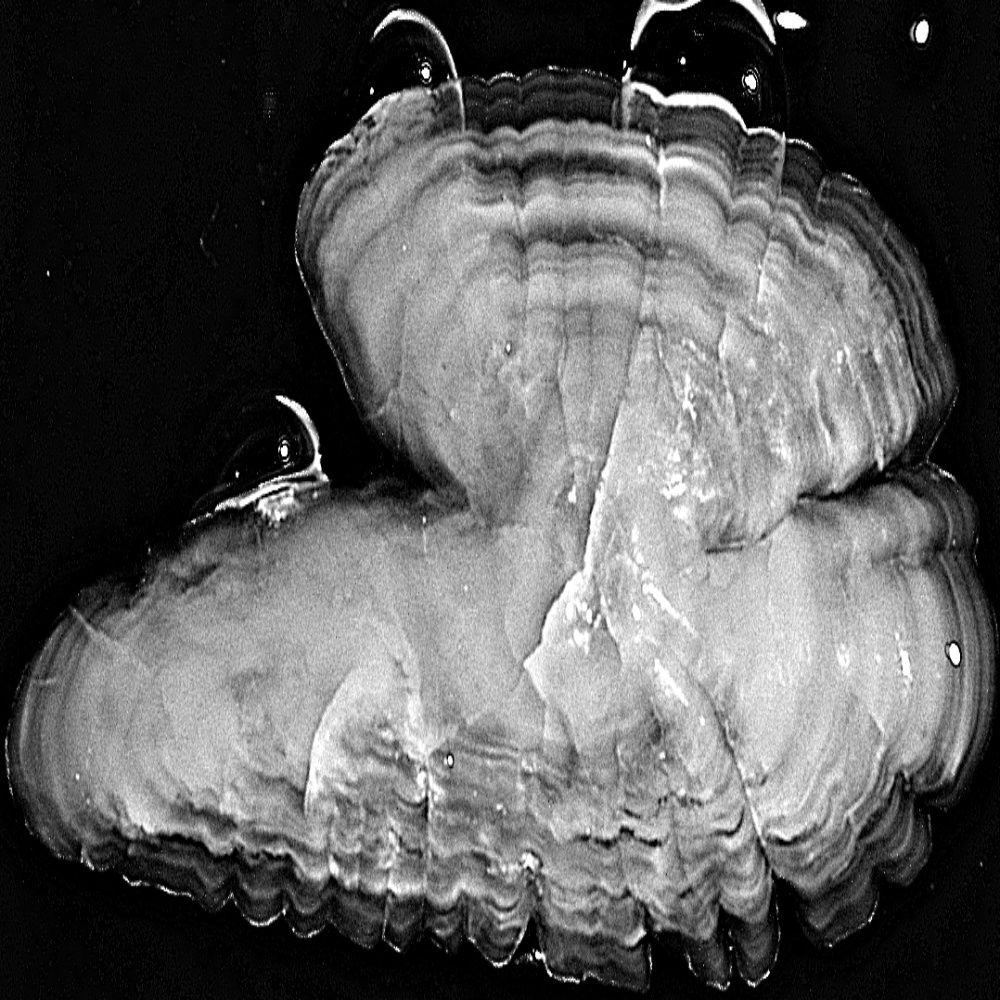
\includegraphics[width=\linewidth]{herring_otolith_example}
    \caption{An example of an otolith image taken from an Atlantic Herring.}
    \label{fig:herring_oto_example}
\end{figure}


\begin{figure}
    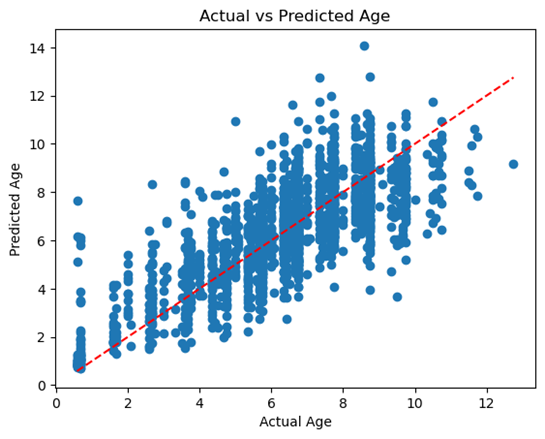
\includegraphics[width=\linewidth]{predict_vs_actual}
    \caption{Actual verses CNN predicted ages of otolith images}
    \label{fig:actual_vs_predicted}
\end{figure}